\documentclass{article}
\usepackage{graphicx}
\usepackage{amsmath} 

\title{\textbf{Theoretical Questions Chapter 4}}
\author{Ling Siu Hong \\ 3200300602}
\begin{document}
\maketitle

\textbf{I} : We have $1\leq m < 2, \beta = 2 , e = \lceil \log_2 477 \rceil = 8$, since
\begin{equation*}
    477 = 2^8 + 2^7 + 2^6 + 2^4 + 2^3 + 2^2 + 2^0 ,
\end{equation*}
therefore
\begin{equation*}
    477 = (1.1101101)_2 \times 2^8 .
\end{equation*}

\textbf{II} : We have $1\leq m < 2, \beta = 2 , e = \lfloor \log \frac{3}{5} \rfloor = -1$, \\
\begin{center}
    $0.6 \times 2 = 1.2  --a_1 = 1 ,$\\
    $0.2 \times 2 = 0.4  --a_2 = 0 ,$\\
    $0.4 \times 2 = 0.8  --a_3 = 0 ,$\\
    $0.8 \times 2 = 1.6  --a_4 = 1 ,$\\
\end{center}

\begin{equation*}
    477 = (1.1101101)_2 \times 2^8.
\end{equation*}


\textbf{III}: Let $x = (1.\overbrace{0000...00}^{p-1 })_{\beta},$
\begin{equation*}
    x_R = (1.\overbrace{0000...01}^{p-1 })_{\beta}\times \beta^e = (1 + \frac{1}{\beta^{p-1}})\ \times \beta^e,
\end{equation*}
\begin{align*}
    x_L =& ((\beta - 1).\overbrace{(\beta - 1)(\beta - 1)...(\beta-1)}^{p-1})_{\beta}  \times \beta^e \\
    =& (\beta - \frac{1}{\beta^{e-1}}) \\
    =& [(\beta - 1 ) + \frac{\beta -1}{\beta} + ... +\frac{\beta -1}{\beta^{p-1}} ]\times \beta^{e-1}. \\
\end{align*}
Since we have $x_R - x = \beta^e + \frac{\beta^e}{\beta^{p-1}} - \beta^e = \beta^{e-p-+1}$ and $x - x_L =  1 \times \beta^{1-p} \times \beta^{e-1}$,thus $x_R - x = \beta(x - x_L).$

\textbf{IV} : Under IEEE754 single-precision, 24 for the significant,
$\frac{3}{5} = (1.0011...)_2 \times 2^{-1} $,the two adjacent are 
\begin{equation*}
    x_R = (1.\overbrace{0011...01}^{23})_2 \times 2^{-1}),
\end{equation*}
\begin{equation*}
    x_L = (1.\overbrace{0011...10}^{23})_2 \times 2^{-1}).
\end{equation*}
Then, we have  $x-x_L = \frac{3}{5} \times 2^{-24}$ ,$x_R - x_L = 1 \times 2^{-24}$,so that $x - x_L > x_R - x$ which means $fl(x) = x_R$.
The relative round off error is 
\begin{equation*}
    \epsilon = \frac{\lvert fl(x) - x \rvert}{\lvert x \rvert} = \frac{2}{3} \times 2{-24} 
\end{equation*}

\textbf{V}: We have $\epsilon_M = \beta^{1-p} $,under IEEE754, $p=24$ and $ \beta = 2$,then $\epsilon_M = 2^{-23}$,
\begin{equation*}
    \epsilon_u = (1-2^{-23})\times \epsilon_M \approx 1.19 \times 10^{-9}
\end{equation*} 

\textbf{VI}
When $x = \frac{1}{4}$, $1-cosx = 0.031087578$, then $2^{-6} \leq 1 - cos(\frac{1}{4}) \leq 2^{-5}$.Therefore, the subtraction will lost at least 5, at most 6 bits of precision.

\textbf{VII}:We can avoid catastrophic cancellation,
\begin{enumerate}
    \item By trigonometric identity 
        \begin{equation*}
            1 - cos x = 2sin^2\frac{x}{2}.
        \end{equation*}
    \item By Taylor's expansion
        \begin{align*}
            1 - cos x =& 1-(1-\frac{x^2}{2!}+\frac{x^4}{4!}-...) \\
            =& \frac{x^2}{2!}-\frac{x^4}{4!} + \frac{x^6}{6!}.
        \end{align*}
\end{enumerate}

\textbf{VIII}
\begin{enumerate}
    \item $f(x) = (x-1)^{\alpha}$
        \begin{equation*}
            C_f(x) = \lvert \frac{x\alpha (x-1)^{\alpha -1}}{(x-1)^{\alpha}} \rvert
        \end{equation*}
    Thus, $C_f \rightarrow \infty$ as $ x \rightarrow 1$
    \item $f(x) = \ln x$
        \begin{equation*}
            C_f(x) = \lvert \frac{1}{\ln x} \rvert
        \end{equation*}
    Thus, $C_f \rightarrow \infty$ as $ x \rightarrow 1$
    \item $f(x) = e^x$
        \begin{equation*}
            C_f(x) = \lvert \frac{x \cdot e^x}{e^x} \rvert = \lvert x \rvert
        \end{equation*}
    Thus, $C_f \rightarrow \infty$ as $ x \rightarrow \infty$
    \item $f(x) = \arccos{x}$
        \begin{equation*}
            C_f(x) = \lvert \frac{x \cdot (-1)}{\sqrt{1-x^2} \arccos{x}} \rvert = \lvert \frac{x}{\sqrt{1-x^2} \arccos{x}} \rvert
        \end{equation*}
    Thus, $C_f \rightarrow \infty$ as $ x \rightarrow \pm 1$
\end{enumerate}

\textbf{IX}
\begin{itemize}
    \item We have $cond_f(x) = \lvert \frac{-xe^{-x}}{1-e^{-x}} \rvert = \lvert \frac{x}{e^x-1}, \rvert$.Let $g(x) = \frac{x}{e^x-1}$,when $x \in (0,1], x < e^x -1$, thus $g(x)\in (0,1]$.
    Since $\lim\limits_{x \to 0}\lvert \frac{x}{e^x-1} \rvert =\lim\limits_{x \to 0}\frac{x}{x+o(x)}=1$ , therefore $cond_f(x) \leq 1$ for $x \in [0,1]$.
    \item Let $f(x) = 1-e^x$, $cond_f(x) = \frac{x}{e^x -1}$,
        \begin{align*}
            f_A(x) =& fl(1-fl(e^-x)) \\
            =& [1-e^{-x}(1+\delta_1)](1+\delta_2),where |\delta_1|\leq \epsilon_u,|\delta_2|\leq \epsilon_u            
        \end{align*}
        Since $\delta_1\delta_2$ is too small, we ignore it then we get
        \begin{equation*}
            f_A(x) = (1-e^{-x})(1 + \delta_2 - \delta_1 \cdot \frac{e^{-x}}{1-e^{-x}})
        \end{equation*}and
        \begin{equation*}
            \phi(x) = 1 + \frac{e^{-x}}{1-e^{-x}} = \frac{1}{1-e^{-x}},
        \end{equation*}
        By theorem 4.76, $cond_A(x) \leq \frac{e^-{x}-1}{x} \cdot \frac{1}{1-e^{-x}} = \frac{e^x}{x}$.
        \item 
            \begin{center}
		  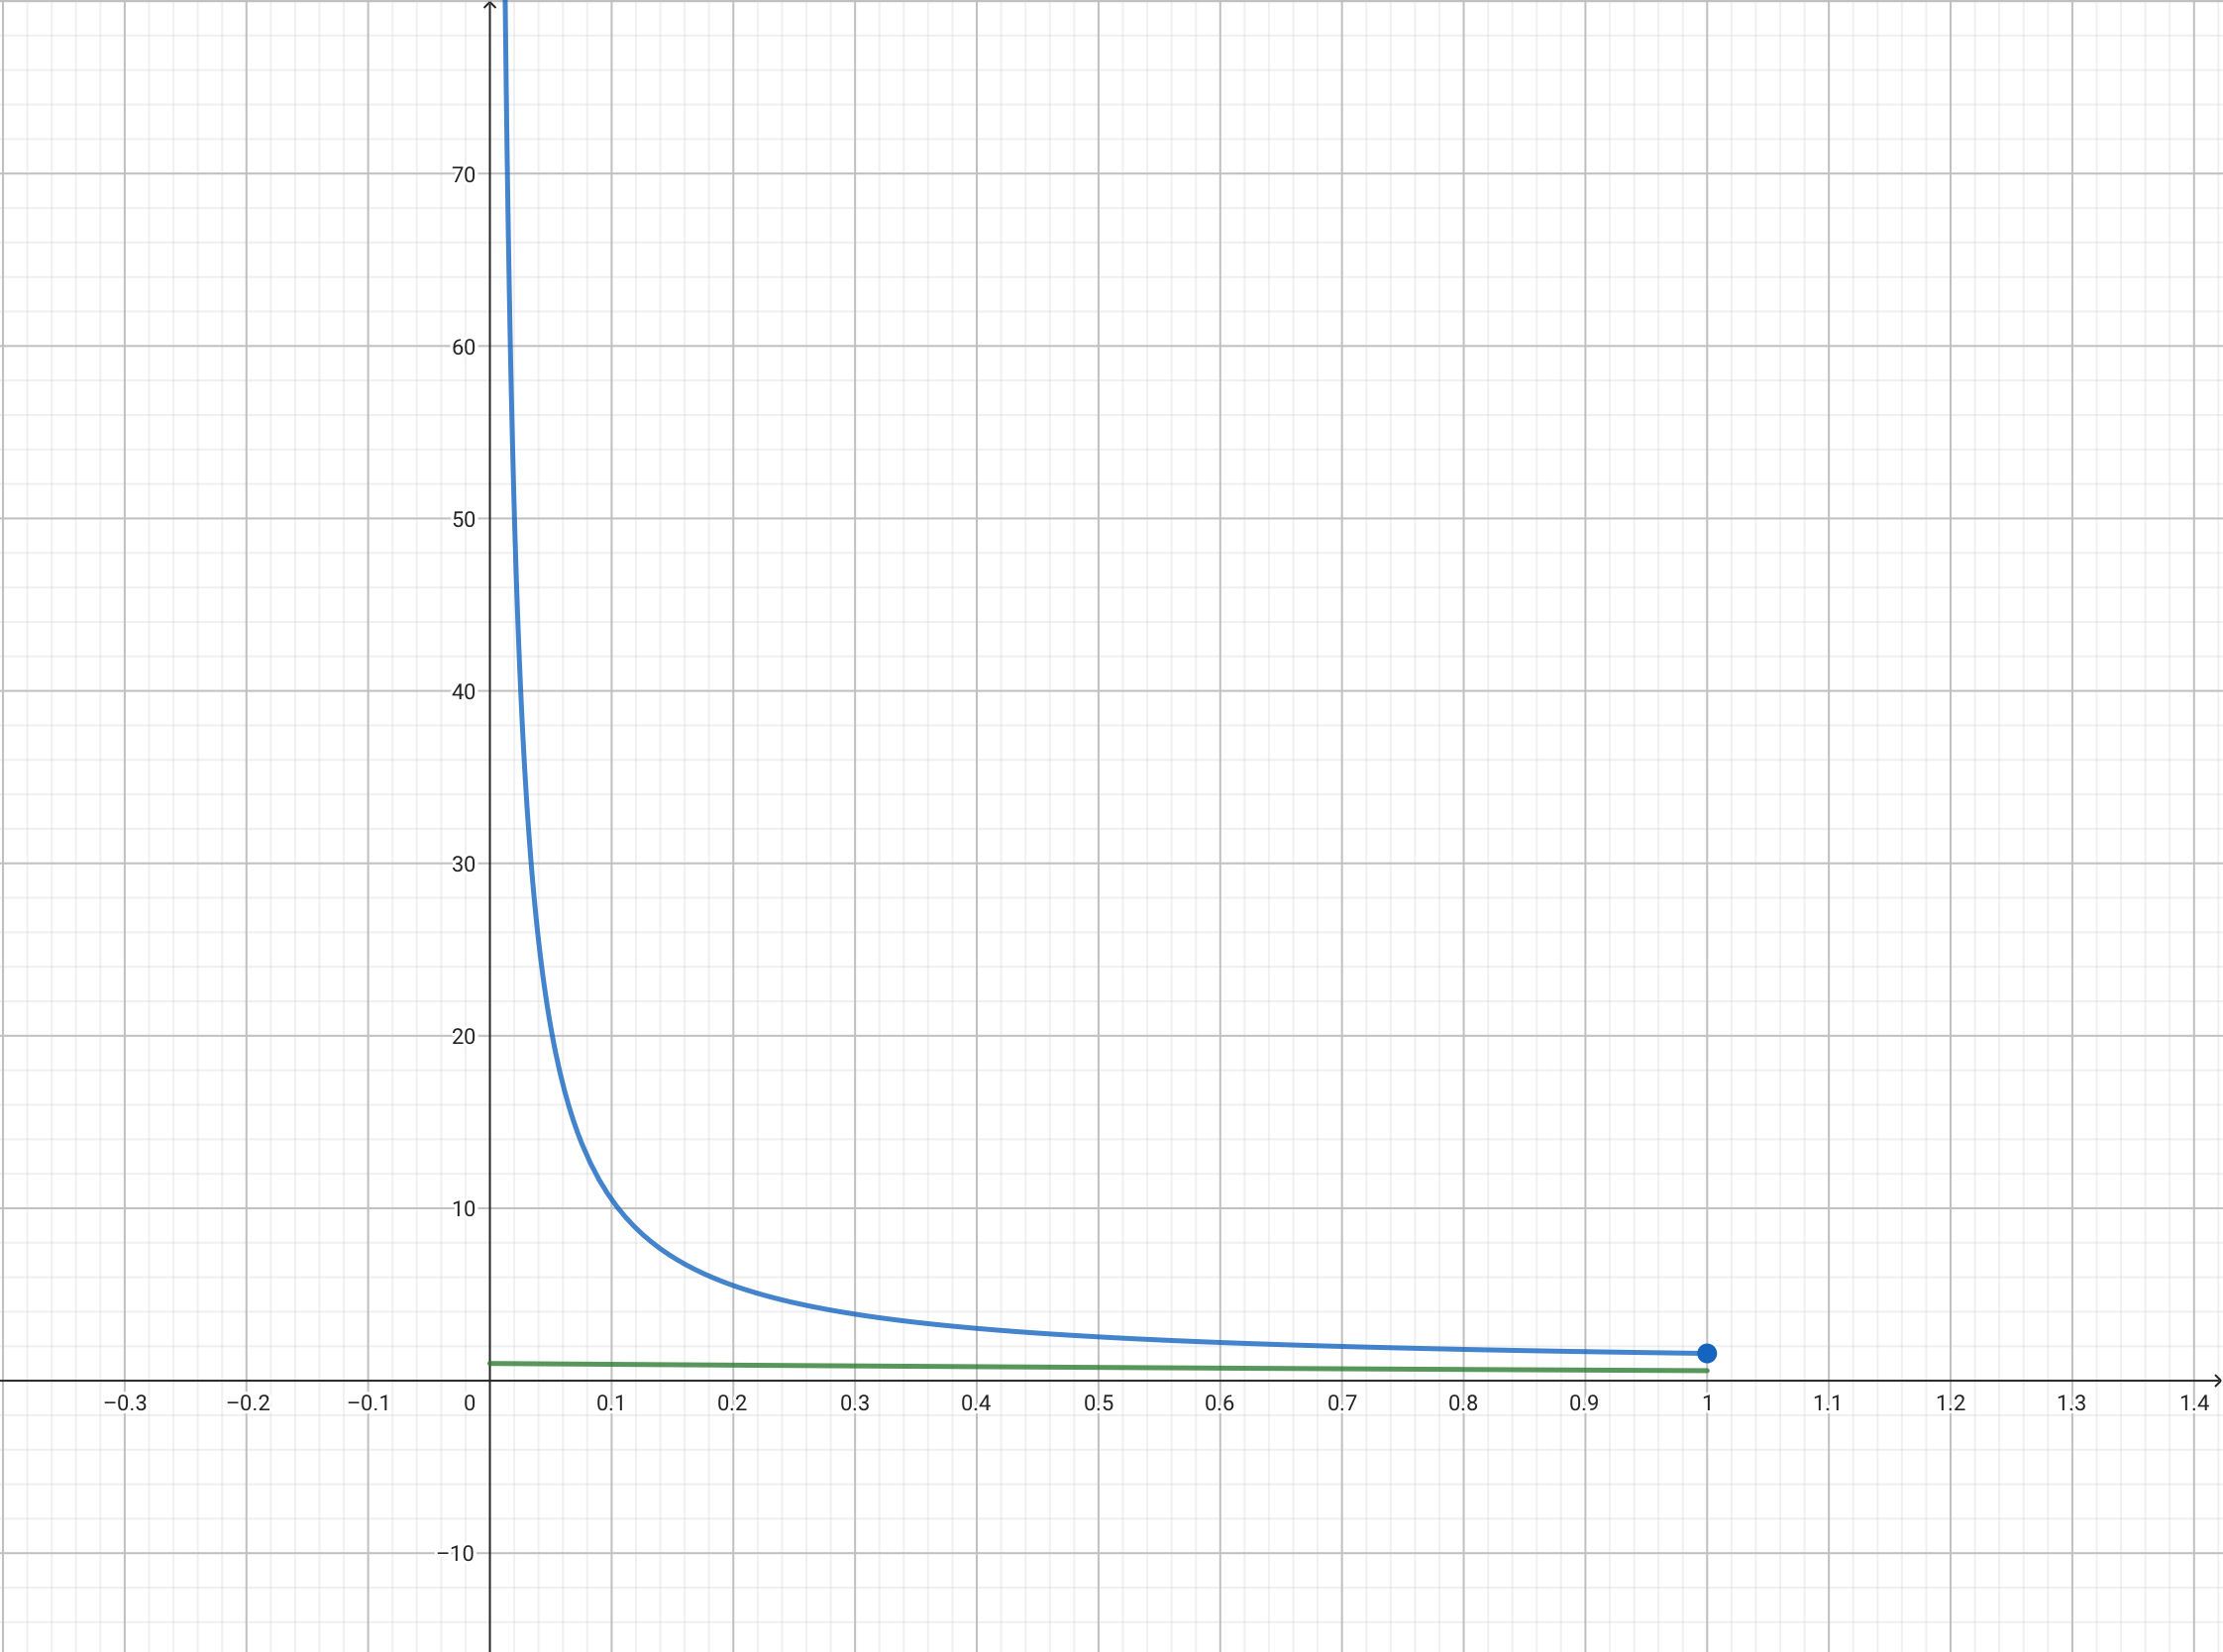
\includegraphics[width=11cm]{picture1.png}	
		  $cond_f(x)$: green; $cond_A(x)$: blue
	      \end{center}
        It is clearly that $cond_A(x)$ if greater than $cond_f(x)$ especially $x \rightarrow 0$. From $cond_A(x) \rightarrow \infty$ as $x\rightarrow 0$, the subtraction $1-e^{-x}$ is not accurate, because $x\rightarrow 0$,$1-e^{-x} \rightarrow 0$.
\end{itemize}

\textbf{X}: Let$r= f(a_0,a_1,...,a_{n-1})$,then we have 
\begin{equation*}
    cond_1=|\frac{1}{r}|\displaystyle\sum_{i=0}^{n-1}|a_i\frac{\partial r}{\partial a_i}|=\frac{\displaystyle\sum_{i=0}^{n-1}|a_ir^i|}{r(\displaystyle\sum_{i=1}^{n}(n-i+1)a_ir^{n-i})}
\end{equation*}
Assume that $r=n$, $f(x)=\displaystyle\prod_{i = 1}^{n}(x-i)$,thus$cond_1=\frac{\displaystyle\prod_{i = 1}^{n}(n+i) -n^n}{n!}$ ,then we have $cond_1 \geq \frac{n^n}{n!}$.
Comparing with Wilkinson, both are $n$ is larger, $cond_1$ will also become larger.

\textbf{XI}: For instance, in FPN system(2,2,-1,1), $a=(1.0)_2 \times 2^0$, $b=(1.1)_2 \times 2^0$.We calculate it in the register of precision 2p(4), and we have $\frac{a}{b} = (0.101)_2$.However,$E_{rel}(\frac{a}{b}) = (0.01)_2 = \epsilon_u$ , contradiction!

\textbf{XII}
Since $128 = (1.000...00)_2 \times 2^7$, $129 = (1.0000001...00)_2 \times 2^7$, thus $2^7 \times 2^-23 = 2^-16 > 10^-6$ ,therefore it cannot compute the root with absolute accuracy $<10^{-6}$.

\textbf{XIII}
{
    Suppose $|x_i,x_i+1| < \delta$, means that the adjacent knot is too close, the cubic spline can be soled by following equation, 
            \begin{align*}             
                a_0 =& f(x_i),\\
                a_0 + \delta a_1 + \delta^2 a_2 + \delta^3 a_3 =& f(x_{i+1}),\\
                a_1 =& f'(x_i),\\
                 a_1 +2\delta a_2 + 3\delta a_3 = &f'(x_{i+1}).
            \end{align*}
    When $\delta \rightarrow 0$,the condition number of coefficient matrix is too large, thus the result is inaccurate.

}
\end{document}
